%
% gausseidel.tex
%
% (c) 2020 Prof Dr Andreas Müller, Hochschule Rapperswil
%
\section{Iterative Gleichungslösung
\label{buch:section:gaussseidel}}
\rhead{Gauss-Seidel-Iteration}
\index{Gleichungssystem!linear}%
\index{lineares!Gleichungssystem}%
Gegeben ist eine lineares Gleichungssystem von $n$ Gleichungen mit
$n$ Unbekannten, welches wir als
\begin{equation}
\begin{linsys}{5}
a_{11}x_1 &+& a_{12}x_2 &+& \dots  \hspace*{7pt}&+& a_{1n}x_n &=& b_1 \\
a_{21}x_1 &+& a_{22}x_2 &+& \dots  \hspace*{7pt}&+& a_{2n}x_n &=& b_2 \\
\vdots\hspace*{5pt}  & & \vdots\hspace*{5pt}  & & \ddots \hspace*{7pt}& & \vdots\hspace*{5pt}  & & \vdots\hspace*{5pt} \\
a_{21}x_1 &+& a_{n2}x_2 &+& \dots  \hspace*{7pt}&+& a_{nn}x_n &=& b_n
\end{linsys}
\label{buch:eqn:linalg:system}
\end{equation}
schreiben.
Abgekürzt wird das Gleichungssystem auch $Ax=b$ notiert, wobei $A=(a_{ij})$
die Koeffizientenmatrix ist, $x=(x_k)$ der Vektor der Unbekannten
und $b=(b_k)$ der Vektor der rechten Seiten.
\index{Koeffizientenmatrix}%

%
% Iterative Lösung
%
\subsection{Iterative Lösung nach Gauss-Seidel
\label{buch:subsection:gauss-seidel}}
Jede der Gleichungen \eqref{buch:eqn:linalg:system} kann nach jeder Variablen
aufgelöst werden, deren zugehöriger Koeffizient von $0$ verschieden ist.
Die Gleichung $k$ in \eqref{buch:eqn:linalg:system} ist
\[
a_{k1}x_1 + a_{k2}x_2 + \dots + a_{kk}x_k + \dots a_{kn}x_n = b_k
\]
Aufgelöst nach $x_k$ ist dies
\[
{\color{red}x_k}
=
\frac1{a_{kk}} (b_k - a_{k1}x_1 - a_{k2}x_2 - \dots - a_{kn}x_n),
\]
sofern $a_{kk}\ne 0$.
Diese Gleichung kann dazu verwendet werden, die Werte für die Unbekannten
zu verbessern.
Wir verwenden daher die Notation $x^{(m)}$ für die $m$-te Approximation
der Lösung.

\begin{satz}[Gauss-Seidel-Iteration]
\index{Gauss-Seidel-Iteration}%
Unter geeigneten Voraussetzungen konvergiert die Folge $x^{(m)}$
definiert durch
\begin{equation}
{\color{red}x_k^{(m)}}
=
\frac{1}{a_{kk}}\bigl(
b_k  - a_{k1}x_1^{(m)} - \dots - a_{k,k-1}x_{k-1}^{(m)}
- a_{k,k+1}x_{k+1}^{(m-1)} - \dots - a_{kn}x_n^{(m-1)}
\bigr)
\label{buch:eqn:gs:iteration}
\end{equation}
mit Startwert $x^{(0)}=0$
gegen die Lösung $x$ des Gleichungssystems $Ax=b$.
\end{satz}

In Abschnitt~\ref{buch:subsection:konvergenzbedingung} werden die
Bedingungen genauer untersucht, die Konvergenz des Verfahrens gegen die
Lösung garantieren können.
\index{Konvergenzbedingung}%

\begin{beispiel}
Sei das Gleichungssystem gegeben durch
\begin{equation}
A=\begin{pmatrix}
2&1&1\\
1&3&1\\
1&1&4
\end{pmatrix}
\qquad\text{und}\qquad
b=\begin{pmatrix}
7\\6\\5
\end{pmatrix}.
\label{buch:eqn:gsbeispiel}
\end{equation}
Die Berechnung der Folge $x^{(m)}$ nach
\eqref{buch:eqn:gs:iteration}
liefert die Werte in Tabelle~\ref{buch:table:gaussseidelbeispiel}.
Die Konvergenz scheint linear zu sein.
\begin{table}
\centering
\begin{tabular}{|>{$}r<{$}|>{$}r<{$}>{$}r<{$}>{$}r<{$}|}
\hline
 m & x_1^{(m)} & x_2^{(m)} & x_3^{(m)} \\
\hline
 0 & 0.0000000             & 0.0000000             & 0.0000000             \\
 1 & 3.5000000             & 0.8333333             & 0.1666667             \\
 2 & 3.0000000             & 0.9444444             & 0.2638889             \\
 3 & \underline{2.8}958333 & \underline{0.94}67593 & \underline{0.2}893519 \\
 4 & \underline{2.88}19444 & \underline{0.94}29012 & \underline{0.29}37886 \\
 5 & \underline{2.88}16552 & \underline{0.941}5187 & \underline{0.294}2065 \\
 6 & \underline{2.882}1373 & \underline{0.941}2187 & \underline{0.2941}610 \\
 7 & \underline{2.8823}102 & \underline{0.94117}62 & \underline{0.2941}284 \\
 8 & \underline{2.8823}476 & \underline{0.94117}47 & \underline{0.29411}94 \\
 9 & \underline{2.882353}1 & \underline{0.94117}59 & \underline{0.294117}7 \\
10 & \underline{2.882353}1 & \underline{0.9411764} & \underline{0.2941176} \\
\hline
\infty&   2.8823529 & 0.9411764 & 0.2941176 \\
\hline
\end{tabular}
\caption{Lösung des Gleichungssystems mit Koeffizientenmatrix $A$ und
rechter Seite $b$ aus \eqref{buch:eqn:gsbeispiel} mit Hilfe des
Gauss-Seidel-Algorithmus.
\index{Gauss-Seidel-Algorithmus}%
In der letzten Zeile die exakten Resultate, erhalten mit dem
Gauss-Algorithmus.
\index{Gauss-Algorithmus}%
\label{buch:table:gaussseidelbeispiel}}
\end{table}
\end{beispiel}


%
% Matrixformulierung
%
\subsection{Matrixformulierung
\label{buch:subsection:matrixformulierung}}
Die Iterationsformel~\eqref{buch:eqn:gs:iteration} verknüpft bei der
Berechnung von $\color{red}x^{(m)}$ Komponenten von $x^{(m-1)}$ und
$\color{red}x^{(m)}$,
\index{Iterationsformel}%
was es etwas schwieriger macht, die Iteration als Fixpunktiteration
der Form ${\color{red}x^{(m)}} = Fx^{(m-1)}$ mit einer
$n\times n$-Matrix $F$ zu schreiben.
\index{Fixpunktiteration}%
\index{Iteration}%
Um dies zu erreichen, zerlegen wir die Matrix $A$ in drei Summanden
$A=L+D+U$, wobei $L$ eine untere Dreiecksmatrix mit Nullen auf der 
Diagonalen sein soll, $D$ eine Diagonalmatrix und $U$ eine obere
Dreiecksmatrix mit  Nullen auf der Diagonalen, also
\begin{align*}
L
&=
\begin{pmatrix}
0        &0        &0        &\dots   & 0         & 0      \\
a_{21}   &0        &0        &\dots   & 0         & 0      \\
a_{31}   &a_{3,2}  &0        &\dots   & 0         & 0      \\
\vdots   &\vdots   &\ddots   &\ddots  & \vdots    & \vdots \\
a_{n-1,1}&a_{n-1,2}&a_{n-1,3}&\dots   & 0         & 0      \\
a_{n1}   &a_{n2}   &a_{n3}   &\dots   & a_{n,n-1} & 0
\end{pmatrix},
\qquad
U
=
\begin{pmatrix}
0      & a_{12} & \dots  & a_{1,n-2} & a_{1,n-1}   & a_{1n} \\
0      & 0      & \dots  & a_{1,n-2} & a_{2,n-1}   & a_{2n} \\
\vdots & \vdots & \ddots & \ddots    &\vdots       & \vdots \\
0      & 0      & \dots  & 0         & a_{n-2,n-1} & a_{n-2,n} \\
0      & 0      & \dots  & 0         & 0           & a_{n-1,n} \\
0      & 0      & \dots  & 0         & 0           & 0
\end{pmatrix}
\intertext{und}
D
&=
\operatorname{diag} (a_{11}, a_{22},\dots , a_{n-1,n-1}, a_{nn}).
\end{align*}
Die Iterationsformel~\eqref{buch:eqn:gs:iteration} lässt sich
mit diesen Matrizen schreiben als
\[
D{\color{red}x^{(m)}} = b - L{\color{red}x^{(m)}} - Ux^{(m-1)}.
\]
Auflösen nach $x^{(m)}$ führt auf
\begin{equation}
{\color{red}x^{(m)}} = (D+L)^{-1} ( b - Ux^{(m-1)} ).
\label{buch:eqn:gs:fixpunkt}
\end{equation}
Die Form \eqref{buch:eqn:gs:fixpunkt} für das Gauss-Seidel-Iterationsverfahren
ist jetzt die einer Fixpunkt-Iteration.

%
% Konvergenzbedingung
%
\subsection{Konvergenzbedingung
\label{buch:subsection:konvergenzbedingung}}
In Kapitel~\ref{chapter:berechnung} haben wir gelernt, dass eine
Fixpunktiteration konvergiert, wenn der Betrag der Ableitung $<1$ ist.
Hier liegt jedoch eine Matrix-Iteration mit der Abbildung
\[
F(x)
=
\underbrace{(D+L)^{-1} b}_{\displaystyle=c} - (D+L)^{-1}U x
=
c - (D+L)^{-1}Ux
\]
vor.
Die Ableitung ist daher ebenfalls eine Matrix, nämlich
\[
D_xF = (D+L)^{-1}U,
\]
und der Fehler der Iteration $m$ ist
\begin{equation}
\delta_m = (D+L)^{-1}U \delta_{m-1}.
\label{buch:gs:fehler}
\end{equation}
Konvergenz kann also nur vorliegen, wenn dieser Vektor im Laufe der
Iteration immer kleiner wird.
\index{Konvergenz}%
Dies ist zum Beispiel dann der Fall, wenn die {\em Norm} der Matrix
kleiner als $1$ ist:
\index{Norm}%

\begin{definition}
Die {\em Norm} einer Matrix $M$ ist
\[
\|M\|
=
\max\{|Mx|\,|\, x\in\mathbb R^n\wedge |x|=1\}.
\]
Für einen Vektor $x\in\mathbb R^n$ gilt $|Mx| \le \|M\|\cdot |x|$.
\end{definition}

Die Bedingung \eqref{buch:gs:fehler} bedeutet jedoch nicht,
dass die Norm der Ableitung $<1$ sein muss, es genügt, wenn
genügend hohe Potenzen der Ableitung eine Norm $<1$ haben.
\index{Ableitung}%

\begin{beispiel}
Die Matrix
\[
M=\begin{pmatrix}
0&2\\
\frac13&0
\end{pmatrix}
\]
hat Norm
\[
\|M\|
=
\max_{|x|=1} |Mx| 
=
\max_{t\in\mathbb R} \sqrt{2^2\cos^2 t +\frac1{3^2}\sin^2t} \ge 2.
\]
Da aber
\[
M^2 = \begin{pmatrix}
\frac{2}{3}&0\\
0&\frac{2}{3}
\end{pmatrix}
\qquad\Rightarrow\qquad \|M^2\|=\frac23
\]
ist, wird eine Iteration mit Ableitungsmatrix $M$ trotzdem
konvergieren, weil der Fehler nach jedem zweiten Schritt um den
Faktor $\frac23$ kleiner geworden ist.
\end{beispiel}

Dies führt uns auf die Grösse
\begin{equation}
\pi(M)
=
\limsup_{n\to\infty} \|M^n\|^\frac1n.
\label{buch:eqn:gelfand-grenzwert}
\end{equation}
Ist $\pi(M) > 1$, dann gibt es Anfangsvektoren $v$ für die Iteration,
für die $M^kv$ über alle Grenzen wächst.
Ist $\pi(M) < 1$, dann wird jeder Anfangsvektor $v$ zu einer Iterationsfolge
$M^kv$ führen, die gegen $0$ konvergiert.
Die Kennzahl $\pi(M)$ erlaubt also zu entscheiden, ob ein
Iterationsverfahren konvergent ist.
\index{Konvergenzbedingung}%

Die Berechnung von $\pi(M)$ als Grenzwert ist sehr unhandlich.
Viel einfacher ist der Begriff des Spektralradius.
\index{Spektralradius}%

\begin{definition}
\label{buch:definition:spektralradius}
Der {\em Spektralradius} der Matrix $M$ ist der Betrag des betragsgrössten
Eigenwertes.
\end{definition}

Wir werden später in Satz~\ref{buch:satz:gelfand} zeigen, dass
$\pi(M) = \varrho(M)$, dies ist bekannt als der Satz von Gelfand.
Um die beiden Begriffe bis dann auseinander halten zu können,
nennen wir den Grenzwert~\ref{buch:eqn:gelfand-grenzwert}
den {\em Gelfand-Radius} $\pi(M)$ der Matrix $M$.
\index{Gelfand-Radius}%
Wir erlauben uns aber, die Überlegungen zu den Iterationsverfahren
mit dem Spektralradius zu formulieren.

Das Gauss-Seidel-Iterationsverfahren ist also genau dann für alle
Startwerte $x_0$ linear konvergent, wenn der Spektralradius
\[
\varrho\bigl( (L+D)^{-1}U \bigr) < 1
\]
ist.
\index{Iterationsverfahren}%

\subsection{Zerlegungsverfahren
\label{buch:subsection:zerlegung}}
\index{Zerlegungsverfahren}%
Das Gauss-Seidel-Verfahren ist nur ein Beispiel einer ganzen Familie
von iterativen Lösungsverfahren für lineare Gleichungssysteme.
Sie basieren alle auf einer Zerlegung $A=B+C$ der Matrix $A$.
Das Gauss-Seidel-Verfahren ist der Fall
\[
A = \underbrace{D+L}_{\displaystyle = B} + \underbrace{R}_{\displaystyle = C}.
\]
Das ursprüngliche Gleichungssystem $Ax=b$ wird jetzt ebenfalls
aufgeteilt in $Bx+Cx=b$.
Ein iteratives Verfahren ergibt sich jetzt dadurch, dass für die beiden $x$
in der Aufteilung verschiedene Iterationen der Lösung verwendet werden,
also $Bx^{(m+1)} + Cx^{(m)} = b$.
Wir erhalten somit das Iterationsverfahren
\begin{equation}
{\color{red}x^{(m+1)}}
=
B^{-1}(b-Cx^{(m)})
=
b_0 - B^{-1}Cx^{(m)}
\end{equation}
Dies ist natürlich nur sinnvoll, wenn sich die Matrix $B$ wesentlich
leichter invertieren lässt als $A$, da andernfalls die Bestimmung von
$x^{(m+1)}$ nicht einfacher ist als die Lösung des ursprünglichen
Gleichungssystems.

Iteriert wird also die Anwendung der Matrix $B^{-1}C$.
Aus der oben entwickelten Theorie lesen wir ab, dass das Zerlgungsverfahren
genau dann konvergiert, wenn der Spektralradius 
$\varrho(B^{-1}C)$ von $B^{-1}C$ kleiner ist als $1$.

\subsubsection{Das Verfahren von Jacobi}
\index{Jacobi-Verfahren}%
Beim Gauss-Seidel-Verfahren wurde jede einzelne Gleichung des
Gleichungssytems nach einer der Variablen aufgelöst und der neue
Wert bei der nächsten Iteration gleich wieder verwendet.
Man hätte natürlich auch erst aus jeder Gleichung einen neuen
Wert für alle Variablen bestimmen können, bevor man diese neuen
Werte in der nächsten Iteration verwendet.
Schreibt man das Gleichungssysten wieder als
\[
(L+D+U) x
=
Lx + D {\color{red}x} + Ux
=
b
\]
dann bedeutet dies, dass man  nach der roten Variablen ${\color{red}x}$
auflöst, also
\[
D{\color{red}x}
=
Lx + Ux + b
\qquad\Rightarrow\qquad
{\color{red}x}
=
D^{-1}(L+U)x + D^{-1}b.
\]
Auch dieses nach {\em Jacobi} benannte Verfahren ist also ein
Zerlegungsverfahren, diesmal mit $B=D$ und $C=L+U$.
Es konvergiert genau dann, wenn $\varrho(D^{-1}(L+U))<1$.
Dieser Fall tritt dann ein, wenn die Diagonalelemente  sehr viel grösser
sind als der Rest der Matrix.

\subsubsection{Richardson-Verfahren}
\index{Richardson-Verfahren}%
Das {\em Richardson-Verfahren} ist besonders gut geeignet für den
Fall, dass die Matrix $A$ nahe an einem Vielfachen der Einheitsmatrix
ist.
\index{Einheitsmatrix}%
Man verwendet dazu die Aufspaltung
\[
A = B + C = \tau E  + (A - \tau E).
\]
Die Matrix $B=\tau E$ ist sehr einfach zu invertieren: $B^{-1}=\frac1\tau E$.
Das Richardson-Verfahren zeichnet sich also durch sehr geringen Aufwand
bei der Invertierung aus.
Die zu iterierende Matrix ist 
\[
B^{-1}C
=
\frac{1}{\tau}E(A-\tau E)
=
\frac1\tau A  - E.
\]
Je näher die Matrix $A$ bei $\tau E$ liegt, desto näher werden die 
Eigenwerte von $A$ bei denen von $\tau E$ also bei $\tau$ liegen,
und desto näher werden die Eigenwerte von $B^{-1}C$ bei $0$ liegen,
was zu Konvergenz des Verfahrens führt.

Die Iterationsformel für die Lösung ist
\index{Iterationsformel}%
\begin{equation}
{\color{red}x}
=
B^{-1}b - B^{-1}Cx
=
\frac1\tau ( b - (A-\tau E)x)
=
\frac1\tau (b-Ax) + x.
\label{buch:richardson-iteration}
\end{equation}
In jedem Schritt wird $x$ also ein Vielfaches von $b-Ax$ korrigiert.
Die Differenz $b-Ax$ misst, um wieviel die Gleichungen nicht 
erfüllt ist, sie heisst auch {\em Residuum}.
\index{Residuum}%

Man kann die Iterationsformel \eqref{buch:richardson-iteration}
auch als eine Variante des Newton-Verfahrens verstehen.
Gesucht wird eine Nullstelle der Funktion $f(x) = b-Ax$.
Das Newton-Verfahren besagt, dass man $x$ um $-Df(x)^{-1}\cdot f(x)$
korrigieren muss.
\index{Newton-Verfahren}%
Allerdings ist $Df(x) = -A$, so dass die Newton-Iterationsformel zu
\[
{\color{red}x}
=
x-
Df(x)^{-1} \cdot f(x)
=
x
+A^{-1}\cdot(b-Ax)
\]
wird.
Genau die Berechnung von $A^{-1}$ soll aber vermieden werden, daher
approxmiert man $A\approx \tau E$, also
\[
{\color{red}x}
=
x
+
\frac{1}{\tau}(b-Ax).
\]
Dies ist wieder die Iterationsformel~\eqref{buch:richardson-iteration}
für das Richardson-Verfahren.
\index{Richardson-Verfahren}%

Im Kapitel~\ref{chapter:cg} wird die Methode der konjugierten Gradienten
vorgeführt.
\index{konjugierte Gradienten}%
Mit ihr lässt sich für symmetrische,
\index{symmetrisch}%
positiv definite Matrizen $A$ ein auf einem Minimalproblem basierendes
\index{positiv definit}%
\index{Minimalproblem}%
iteratives Verfahren konstruieren lässt, welches ebenfalls genau
die Residuen als Verbesserungsrichtungen für die Lösung verwendet.

\subsubsection{Successive Overrelaxation (SOR)}
\index{successive overrelaxation}%
\index{SOR}%
Das Gauss-Seidel-Verfahren versucht jede einzelne Variable
ohne Rücksicht auf alle anderen zu korrigieren.
\index{Gauss-Seidel-Verfahren}%
Die einzelne Korrektur soll also den ganzen verbleibenden Fehler
ausbügeln.
Es ist klar, dass diese Korrektur zwar ungefähr in die richtige
Richtung erfolgt, aber nicht vom richtigen Betrag sein wird.
Das Richardson-Verfahren enthält einen Parameter, mit dem man die Konvergenz
beeinflussen kann.
\index{Richardson-Verfahren}%
Man muss also versuchen, das Ausmass der Korrektur im Gauss-Seidel-Verfahren
zu parametrisieren und den Parameter so zu wählen, dass die
Konvergenzgeschwindigkeit optimiert werden kann.

In einem Iterationsschritt des Gauss-Seidel-Verfahrens wird die Variable
$x_k$ durch
\[
{\color{red}x_k}
=
\frac1{a_{kk}}\biggl( b_k - \sum_{i\ne k} a_{ki}x_i\biggr)
\]
ersetzt, also um den Betrag
\[
\delta_k
=
{\color{red}x_k} - x_k
=
\frac1{a_{kk}}\biggl(b_k-\sum_{i\ne k} a_{ki}x_i\biggr) - x_k
\]
korrigiert.
Statt um $\delta_k$ korrigieren wir jetzt um $\omega\delta_k$, also auf
\[
{\color{red}x_k}
=
x_k 
+
\omega
\biggl(\frac1{a_{kk}}\biggl( b_k - \sum_{i\ne k} a_{ki}x_i\biggr) - x_k\biggr).
\]
Wie im Gauss-Seidel-Verfahren werden die korrigierten Variablen bereits
bei der nächsten Gleichung wieder verwendet, es ist also
\[
{\color{red}x_k}
=
x_k
+
\omega\biggl(
\frac1{a_{kk}}\biggl(b_k - \sum_{i=1}^{k-1} a_{ki}{\color{red}x_i}
- \sum_{i=k+1}^n a_{ki}x_i\biggr)-x_k\biggr)
\biggr).
\]
In Matrixform geschrieben wird dies zu
\[
{\color{red}x}
=
x
+\omega
(
D^{-1}
(b - L{\color{red}x} - Ux)
-x
).
\]
Nach Multiplikation von links mit $D$ erhalten wir
\[
D{\color{red}x}
=
Dx + \omega b - \omega L{\color{red}x} - \omega Ux - \omega Dx.
\]
Um den Zusammenhang mit den Zerlegungsverfahren herzustellen, dividieren
wir durch $\omega$ und bringen alle Terme mit $x$ und $\color{red}x$
auf die linke Seite, was
\begin{align*}
\frac1\omega D{\color{red}x} 
-
\frac1\omega Dx
+
L{\color{red}x}
+
Ux
+
Dx
&=
b
\intertext{ergibt. Dies können wir etwas klarer als}
\underbrace{
\biggl(
L
+
\frac1\omega D
\biggr)}_{\displaystyle =B_\omega}{\color{red}x}
+
\underbrace{\biggl(
U+\biggl(1-\frac1\omega\biggr)D
\biggr)}_{\displaystyle =C_\omega}
x
&=
b
\end{align*}
umordnen.
Wir haben damit ein Zerlegungsverfahren basierend auf der Zerlegung
$A=B_\omega+C_\omega$
gefunden.

Die Korrektur der Variablen $x_k$ nach Gauss-Seidel wird oft
Relaxation genannt.
\index{Relaxation}%
Ein Parameter-Wert $\omega >1$ führt eine grössere Korrektur aus,
man bezeichnet dies als Überrelaxation.
\index{Überrelaxation}
Die Korrektur wird wie beim Gauss-Seidel-Verfahren
nacheinander auf alle Variablen angewendet wird, daher heisst dieses
Verfahren {\em Successive Overrelaxation} oder kurz SOR.
\index{sukzessiv}%
Geignete Werte von $\omega$ liegen zwischen $0$ und $2$,
das Gauss-Seidel-Verfahren ist der Fall $\omega = 1$.
Man kann zeigen, dass dieses Verfahren für symmetrische Matrizen
immer konvergiert.

\begin{table}
\centering
\renewcommand\arraystretch{1.8}
\begin{tabular}{l>{$}l<{$}>{$}l<{$}>{$}l<{$}}
Methode      & B      & C        & \text{Iterationsformel} \\
\hline
Jacobi       & D      & L + U    & {\color{red}x} = D^{-1}b - D^{-1}(L+U)x \\
Gauss-Seidel & D+L    & U        & {\color{red}x} = (D+L)^{-1}b- (D+L)^{-1}Ux \\
Richardson   & \tau E & A-\tau E & {\color{red}x} = \displaystyle \frac1\tau (b-Ax)+x\\
SOR          & \displaystyle B_\omega=\frac1\omega D + L
                      & \displaystyle C_\omega=\biggl(1-\frac1\omega\biggr)D+U
                                 & {\color{red}x} = B_\omega^{-1}b - B_\omega^{-1}C_\omega x 
\\[3pt]
\hline
\end{tabular}
\caption{Zusammenstellung iterativer Verfahren für die Lösung eines
Gleichungssystems $Ax=b$, welche auf einer Zerlegung der Matrix $A$
in $A=B+C$ basieren.
\label{buch:table:liniteration}}
\end{table}
Tabelle~\ref{buch:table:liniteration} stellt die in diesem Abschnitt
beschriebenen, auf dem Zerlegungsprinzip basierenden Verfahren zusammen.

\begin{beispiel}
Zur Illustration berechnen wir die verschiedenen Spektralradien für
eine symmetrische $30\times 30$-Matrix der Form $E + R$,
wobei $R$ aus zufälligen Werten
im Intervall $[0,0.1]$ besteht.
In einer typischen Rechnung ergaben sich die Werte
\[
\begin{aligned}
\text{Gauss-Seidel:}&&
\varrho((D+L)^{-1}U) &=  0.29160
&&\text{konvergiert}
\\
\text{Jacobi:}&&
\varrho(D^{-1}(L+U)) &=  1.3724
&&\text{konvergiert nicht.}
\end{aligned}
\]
\begin{figure}
\centering
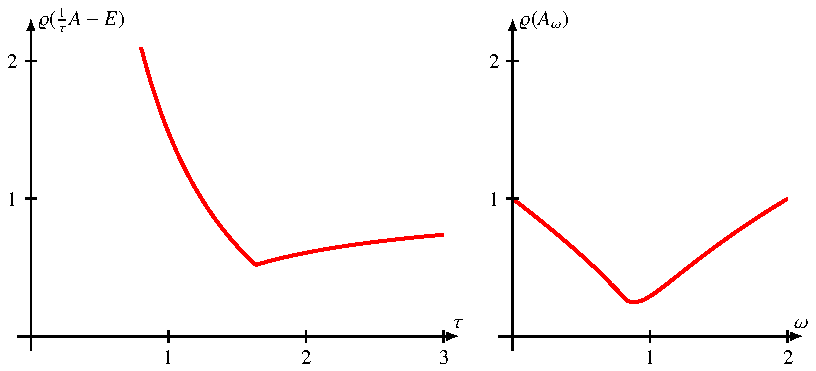
\includegraphics{chapters/60-linsys/images/sp.pdf}
\caption{Spektralradius für das Richardson-Verfahren in Abhängigkeit
von $\tau$ und für SOR in Abhängigkeit von $\omega$.
In beiden Fällen gibt es einen Parameterwert, für den die
Konvergenzgeschwindigkeit maximal ist.
\label{buch:figure:spektralradius}}
\end{figure}%
In Abbildung~\ref{buch:figure:spektralradius}
ist der Spektralradius der Iterationsmatrix für
das Richardson-Verfahren und für SOR dargestellt.
In beiden Fällen gibt es einen Wert für den Parameter,
für den der Spektralradius minimal und damit die Konvergenzgeschwindigkeit
am grössten wird.
\index{Konvergenzgeschwindigkeit}%
Es stellt sich heraus, dass das SOR-Verfahren in diesem speziellen Fall
für ein $\omega<1$ am schnellsten konvergiert, also für Unterrelaxation.
\end{beispiel}



